\documentclass[letterpaper,12pt]{article}
\usepackage{graphicx}
%\extrafloats{100}%
\graphicspath{ {figures/} }
\author{Juliana Pulsinelli}
\title{Benchmarking of the Non-Relativistic Hydrodynamics Alogorithms in thornado}
\begin{document}
\maketitle
\begin{abstract}

The thornado project is astrophysical code based on the Euler equations for fluid dynamics. In this project, the algorithms were benchmarked for accuracy. A group of one-dimensional Riemann problems with known exact solutions were run, and the thornado results were graphed and compared to the exact solutions. 

\end{abstract}
\section{Introduction}
Astrophysical fluid dynamics models the movement of fluids in space. It yields very different solutions from terrestrial fluid dynamics, as the effect of gravity is reduced or removed. 
Fluid dynamics play a major role in the formation of stars and neutron stars, as well as the movement of galaxies and numerous other astrophysical topics.  

In this project, algorithms solving the Euler equations for fluid dynamics were tested using a variety of tests. The Euler equations for fluid dynamics are \cite{ZhangShu2010}:


\begin{equation}
	\frac{\partial \rho}{\partial t}  
	+ \frac{\partial}{\partial x} \Big(\rho u\Big) = 0
\end{equation}

\begin{equation}
	\frac{\partial}{\partial t} \Big(\rho u\Big)
	+ \frac{\partial}{\partial x} \Big(\rho u^2 + p\Big) = 0
\end{equation}

\begin{equation}
	\frac{\partial E}{\partial t}
	+ \frac{\partial}{\partial x} \Big((E + p) u\Big) = 0
\end{equation}

\begin{equation}
	p = (\gamma - 1)
	\Big(E - \frac{1}{2} \rho u^2 \Big)
\end{equation}

where $\rho$ represents mass density, u represents fluid velocity, p represents pressure of the fluid, and E represents energy. 
Equation 1 represents conservation of mass, equation 2 represents conservation of momentum, and equation 3 represents conservation of energy. Equation 4 is the equation of state, which links the other three equations. 

The code was tested using Riemann problems. The Riemann problem models a fluid in an area of one-dimensional space. The initial data features one jump discontinuity, and is constant on either side of this discontinuity. The computational domain is divided into space and time cells. The conditions of each cell are advanced forward for all space cells, one time step at a time, according to the Euler equations for fluid dynamics. \cite{Leveque2002}

%models an area with two fluids, each of which has different characteristics, which are separated from one another by a barrier. When the barrier is removed, the Riemann problem solver code models how the fluids mix, determining how different properties of the fluid change at various spatial locations over time. The fields are evolved forward over time based on the Euler equations.

\section{Numerical Experiments}
Several tests were used to assess the accuracy of the integration method \cite{LiskaWendroff2003}. 
\begin{table}
\begin{center}
\begin{tabular}{ |c|c c c|c c c|c c| }
 \hline
 Test & $\rho_L$ & $u_L$ & $p_L$ & $\rho_R$ & $u_R$ & $p_R$ & $x_0$ & T \\
 \hline
 1 & 1 & 0 & 1 & 0.125 & 0 & 0.1 & 0.5 & 0.2 \\
 2 & 1 & 0.75 & 1 & 0.125 & 0 & 0.1 & 0.3 & 0.2 \\
 3 & 1 & -2 & 0.4 & 1 & 2 & 0.4 & 0.5 & 0.15 \\
 4 & 1 & 1 & $10^-6$ & 1 & -1 & $10^-6$ & 0.5 & 1 \\
 5 & 1 & -19.59745 & 1000 & 1 & -19.59745 & 0.01 & 0.8 & 0.012 \\
 6 & 5.99924 & 19.5975 & 460.894 & 5.99242 & -6.19633 & 46.095 & 0.4 & 0.035 \\
 7 & 1.4 & 0 & 1 & 1 & 0 & 1 & 0.5 & 2 \\
 8 & 1.4 & 0.1 & 1 & 1 & 0.1 & 1 & 0.5 & 2 \\
 9 & 0.1261192 & 8.9047029 & 782.92899 & 6.591493 & 2.2654207 & 3.1544874 & 0.5 & 0.0039 \\
10 & 5.6698 & 9.0299 & 100 & 1.0 & 0.0 & 1.0 & 0 & ? \\
11 & 5.6698 & −1.4701 & 100 & 1.0 & -10.5 & 1.0 & 0 & ? \\
 \hline
\end{tabular}
  \caption{table of tests}
  \label{tab:testtable}
\end{center}
\end{table}
$x_0$ refers to the position of the barrier. The computational domain is 0.0 to 1.0 in tests 1--8, 0.1 to 0.6 in test 9 \cite{LiskaWendroff2003}, -5 to 15 in test 10, and -15 to 5 in test 11 \cite{Leveque2002}. 

Test 12 is an interacting blast waves test, computed on 0.0 to 1.0, with discontinuities at 0.1 and 0.9. At all positions, initial density is 1 and initial velocity is 0. Initial pressure is 1000 on the left, 0.01 in the center, and 100 on the right \cite{LiskaWendroff2003}.

\subsection{Test 1: Sod's Shock Tube} 

First, the tests were run with values computed at different intervals; the method of integration is the same in each test. Between the two endpoints, 128, 256, 512, and 1024 points were computed for on each respective test. Figures~\ref{fig:dencellcomp_20}--\ref{fig:velcellcomp_20} show results of these tests:
\begin{figure}
  \begin{center}
    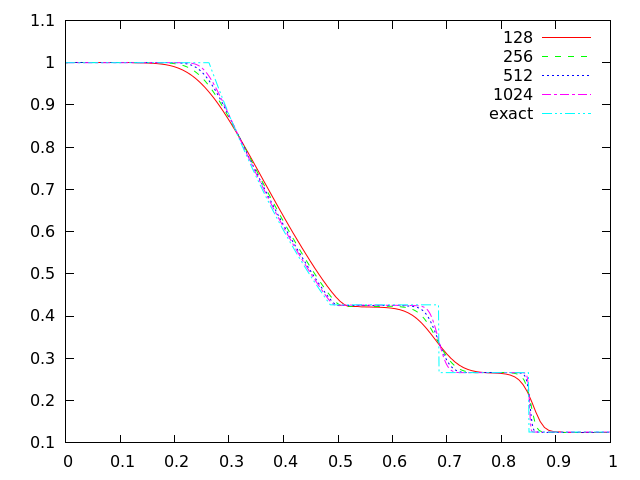
\includegraphics[width=.95\textwidth]{dencellcomp_20}
  \end{center}
  \caption{density}
  \label{fig:dencellcomp_20}
\end{figure}
%\newpage 

\begin{figure}
  \begin{center}
	\begin{tabular}{cc}
      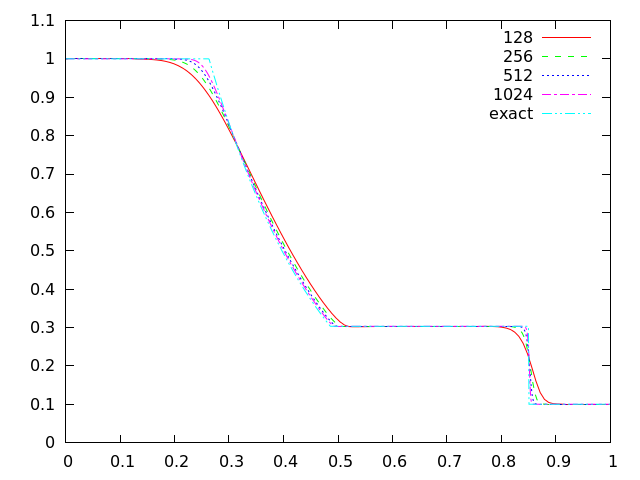
\includegraphics[width=.425\textwidth]{prscellcomp_20} &
	  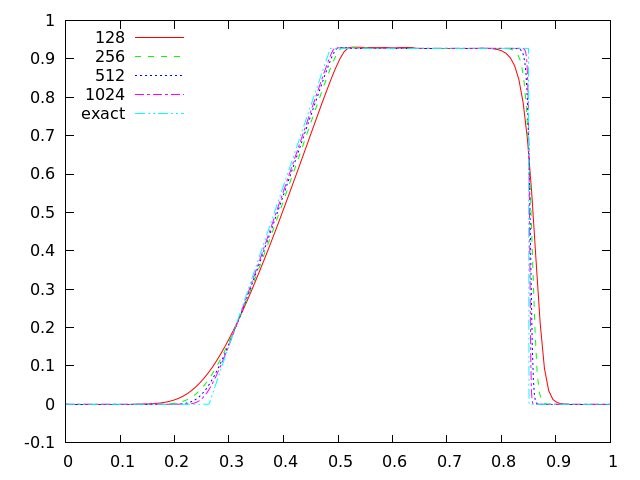
\includegraphics[width=.425\textwidth]{velcellcomp_20}
	\end{tabular}
  \end{center}
  \caption{pressure and velocity}
\end{figure}
%\newpage

%\clearpage
%\begin{figure}
 % \begin{center}
    
 % \end{center}
 % \caption{velocity}
 % \label{fig:velcellcomp_20}
%\end{figure}
%\clearpage
Next, several tests were run of different integration methods; the number of points was held constant at 128 each time. Higher numbers in the key correspond to higher-order, more exact methods of integration. 

\begin{figure}[h]
  \begin{center}
    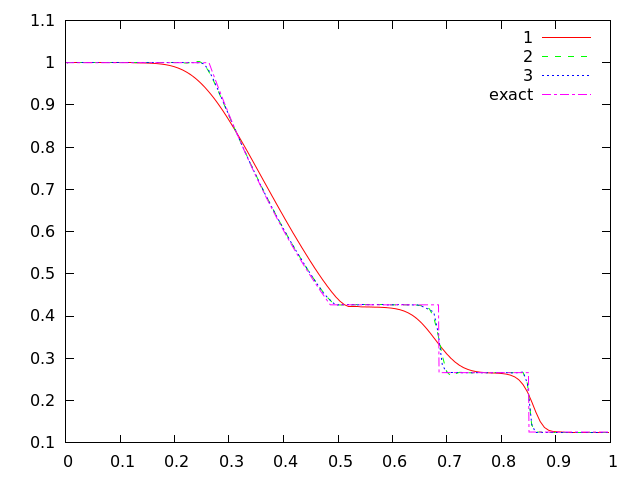
\includegraphics[width=.78\textwidth]{den128comp_20}
  \end{center}
  \caption{density}
\end{figure}
%\newpage

\begin{figure}
  \begin{center}
	\begin{tabular}{cc}
      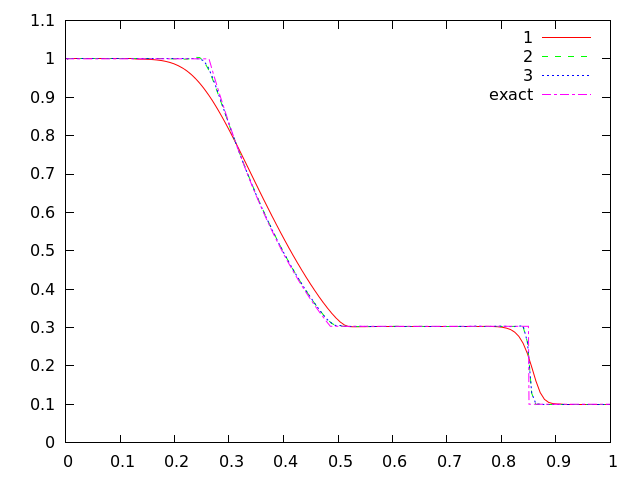
\includegraphics[width=.425\textwidth]{prs128comp_20} &
	  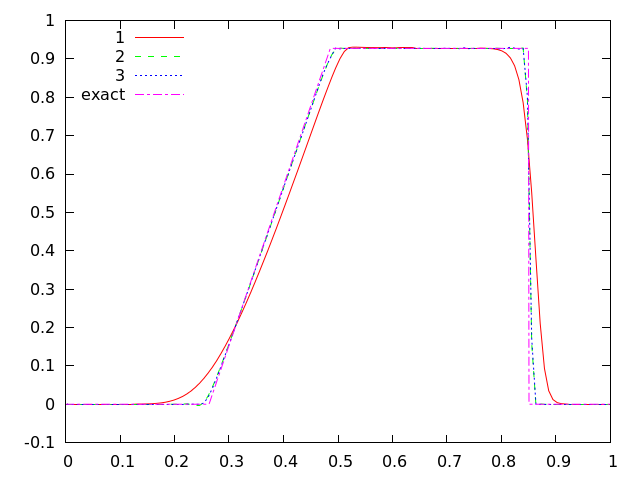
\includegraphics[width=.425\textwidth]{vel128comp_20}
	\end{tabular}
  \end{center}
  \caption{pressure and velocity}
\end{figure}


These graphs show that the combination of both the lowest order integration method and 128 points yields significant error; however, improving either the method of integration or the number of points gives a solution much closer to the exact solution. 

\clearpage

\subsection{Test 2}
For subsequent tests, the number of cells was consistent within each test, and the integration method was varied as in the first test. 
The graphs for the second test show a result common throughout many of the different tests: The first order integration method is considerably far from the exact solution; the second and third order integration methods yield nearly identical results which are near, but not exactly equal to, the exact solution. 
\begin{figure}[h]
  \begin{center}
     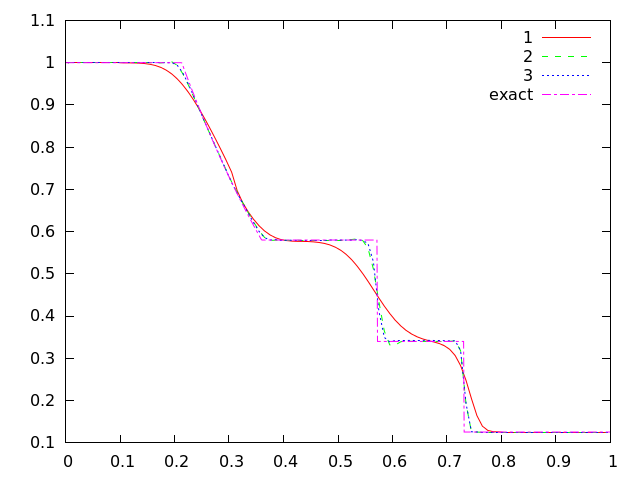
\includegraphics[width=.78\textwidth]{den_T2.png}	
  \end{center}
  \caption{density}
\end{figure}

\begin{figure}
  \begin{center}
	\begin{tabular}{cc}
      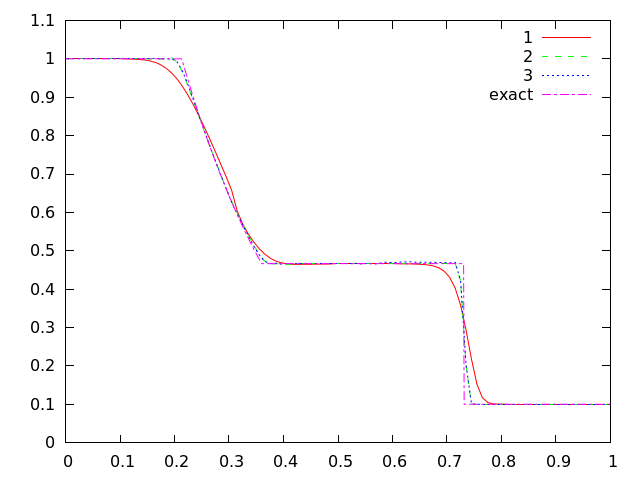
\includegraphics[width=.425\textwidth]{prs_T2.png} &
	  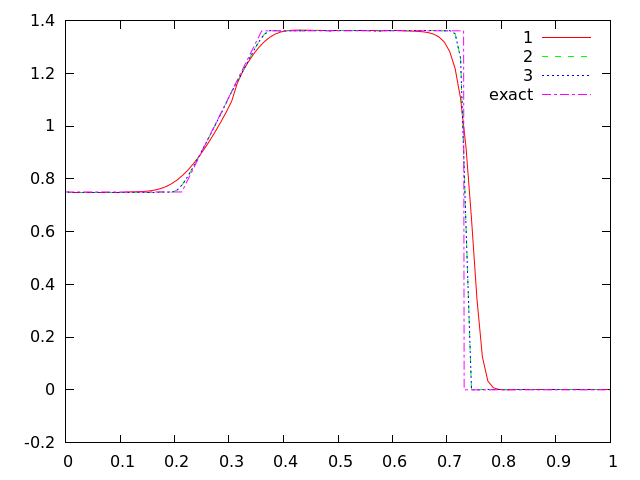
\includegraphics[width=.425\textwidth]{vel_T2.png}
	\end{tabular}
  \end{center}
  \caption{pressure and velocity}
\end{figure}


\clearpage

\subsection{Test 3}
Test 3 shows results similar to Test 2. The deviation of experimental results from exact is especially noticeable in velocity. Near the initial point of discontinuity, the exact results appear completely horizontal. Method 1 almost completely ignores this horizontal part, while Methods 2 and 3 smooth it out considerably. 
\begin{figure}[h]
  \begin{center}
     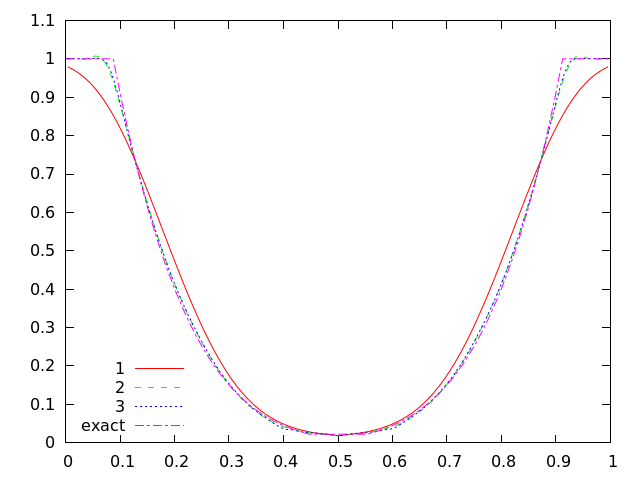
\includegraphics[width=.78\textwidth]{den_T3.png}	
  \end{center}
  \caption{density}
\end{figure}

\begin{figure}
  \begin{center}
	\begin{tabular}{cc}
      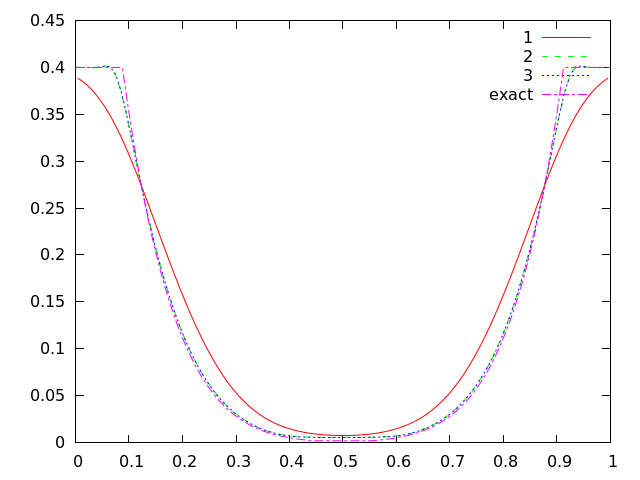
\includegraphics[width=.425\textwidth]{prs_T3.png} &
	  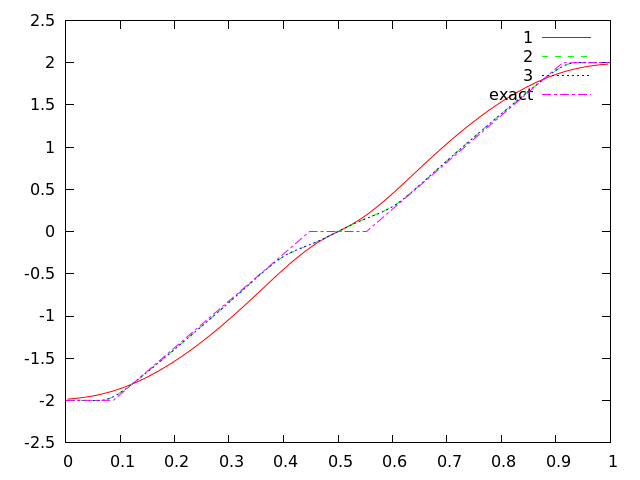
\includegraphics[width=.425\textwidth]{vel_T3.png}
	\end{tabular}
  \end{center}
  \caption{pressure and velocity}
\end{figure}

\clearpage

\subsection{Test 4}

This test obviously displays some difference from the exact solution in density. A depression appears in the center of the graph which is not part of the exact solution. This depression is most severe when method 1 is used, but it also appears with methods 2 and 3. 

\begin{figure}[h]
  \begin{center}
     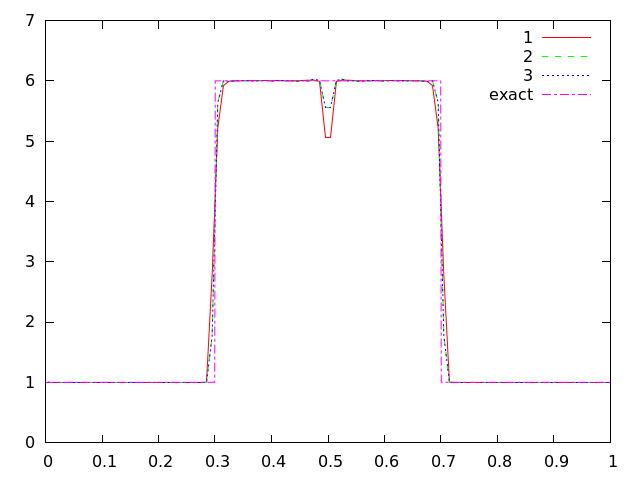
\includegraphics[width=.78\textwidth]{den_T4.png}	
  \end{center}
  \caption{density}
\end{figure}

\begin{figure}
  \begin{center}
	\begin{tabular}{cc}
      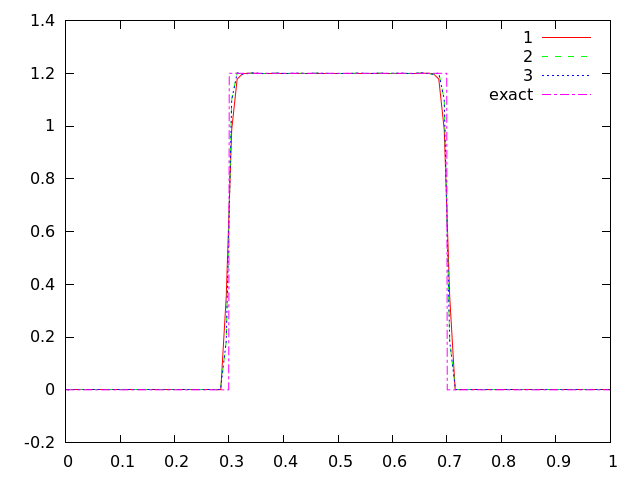
\includegraphics[width=.425\textwidth]{prs_T4.png} &
	  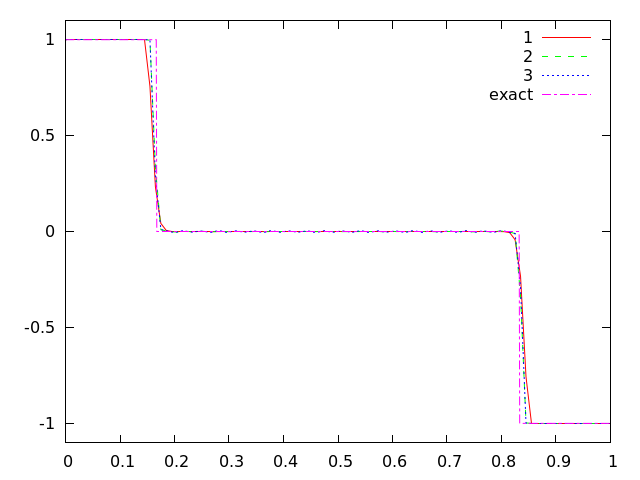
\includegraphics[width=.425\textwidth]{vel_T4.png}
	\end{tabular}
  \end{center}
  \caption{pressure and velocity}
\end{figure}

\clearpage

\subsection{Test 5}
This test has interesting features in velocity. The first integration method underestimates the velocity at positions between about 0.2 and 0.5. The second and third order methods find a bump in density at around 0.4, which is not present in the exact solution.

\begin{figure}[h]
  \begin{center}
     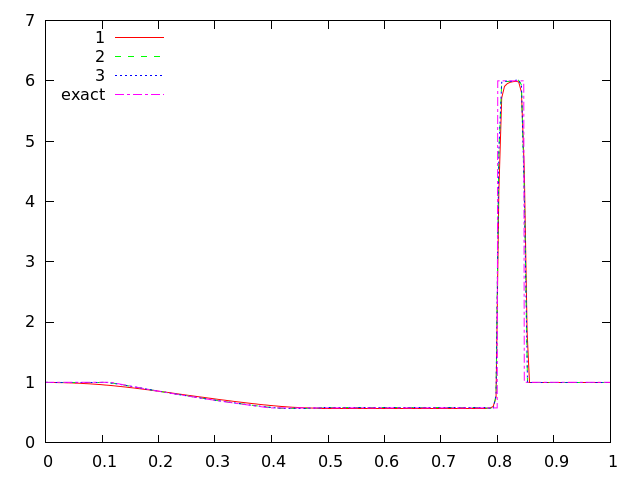
\includegraphics[width=.78\textwidth]{den_T5.png}	
  \end{center}
  \caption{density}
\end{figure}

\begin{figure}
  \begin{center}
	\begin{tabular}{cc}
      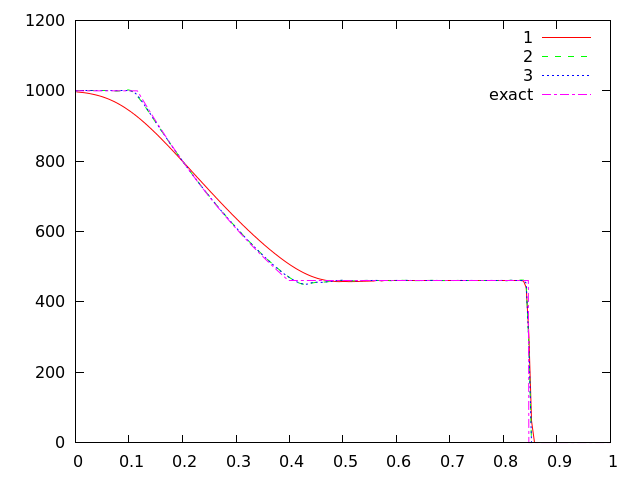
\includegraphics[width=.425\textwidth]{prs_T5.png} &
	  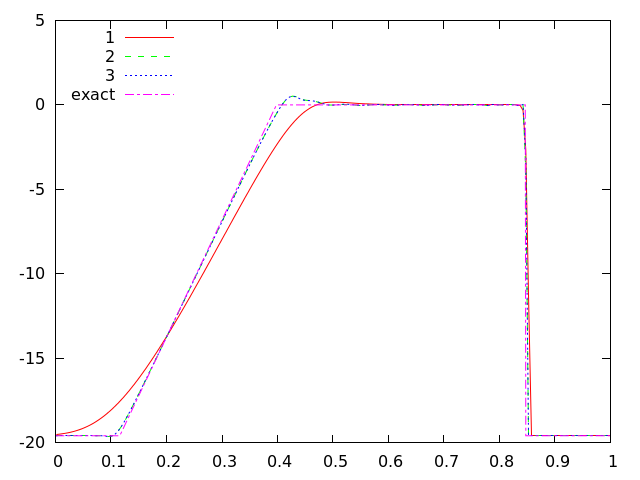
\includegraphics[width=.425\textwidth]{vel_T5.png}
	\end{tabular}
  \end{center}
  \caption{pressure and velocity}
\end{figure}
\clearpage

\subsection{Test 6}
For this test's pressures and velocity, all three integration methods give values very close to exact. However, method 1 proves to be quite bad--worse than usual--at computing the density for this test. 

\begin{figure}[h]
  \begin{center}
     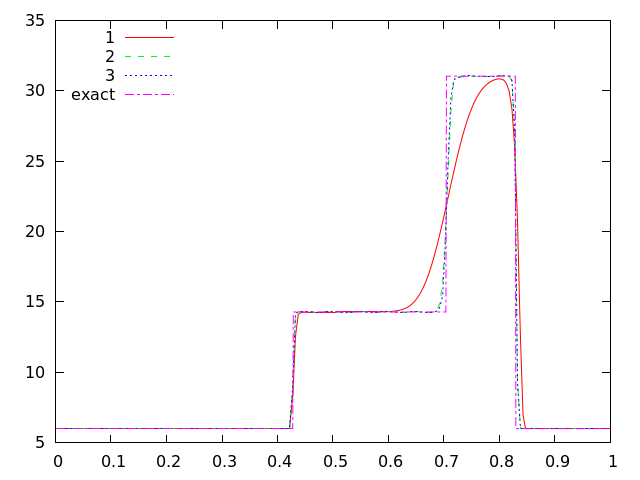
\includegraphics[width=.78\textwidth]{den_T6.png}	
  \end{center}
  \caption{density}
\end{figure}

\begin{figure}
  \begin{center}
	\begin{tabular}{cc}
      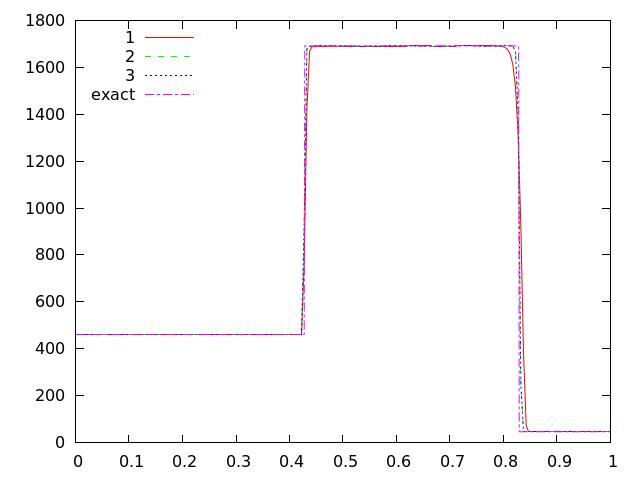
\includegraphics[width=.425\textwidth]{prs_T6.png} &
	  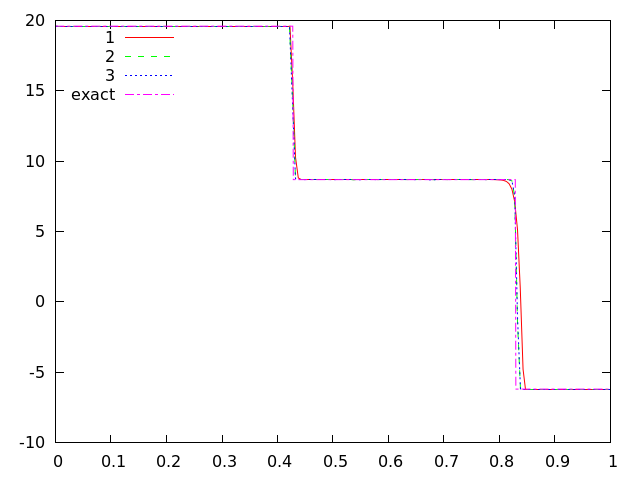
\includegraphics[width=.425\textwidth]{vel_T6.png}
	\end{tabular}
  \end{center}
  \caption{pressure and velocity}
\end{figure}

\clearpage

\subsection{Test 7}
This test features an unusual situation--method 1 calculates the velocity exactly, while method 2 introduces more error and method 3 introduces the most. However, this graph only appears extreme because the intervals on its axis are so small. The numbers are always very close to zero, but very slight errors occur in some of the computations. 

\begin{figure}[h]
  \begin{center}
     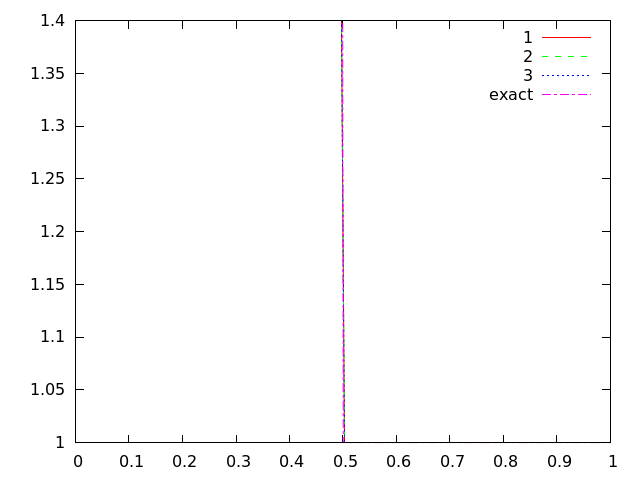
\includegraphics[width=.78\textwidth]{den_T7.png}	
  \end{center}
  \caption{density}
\end{figure}

\begin{figure}
  \begin{center}
	\begin{tabular}{cc}
      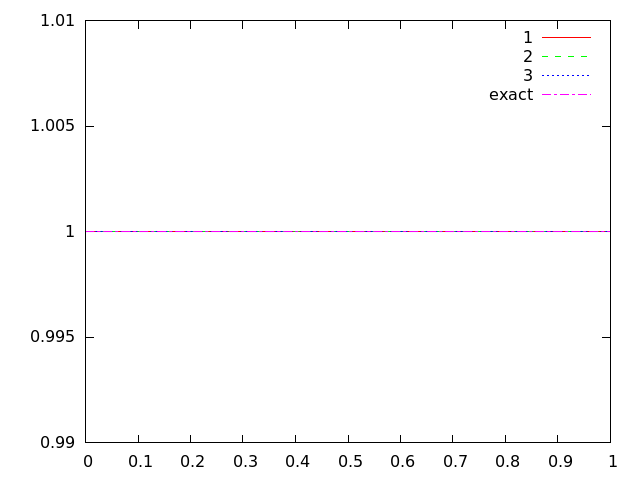
\includegraphics[width=.425\textwidth]{prs_T7.png} &
	  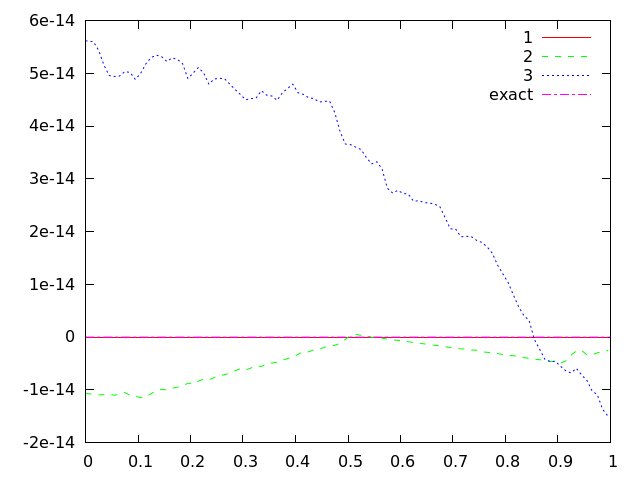
\includegraphics[width=.425\textwidth]{vel_T7.png}
	\end{tabular}
  \end{center}
  \caption{pressure and velocity}
\end{figure}

\clearpage

\subsection{Test 8}

\begin{figure}[h]
  \begin{center}
     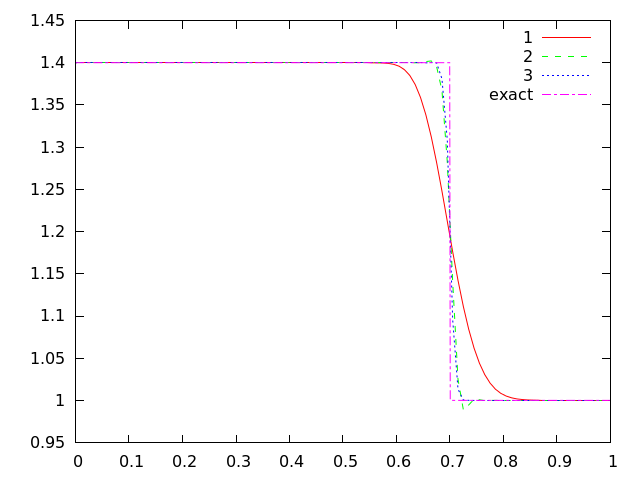
\includegraphics[width=.78\textwidth]{den_T8.png}	
  \end{center}
  \caption{density}
\end{figure}

\begin{figure}
  \begin{center}
	\begin{tabular}{cc}
      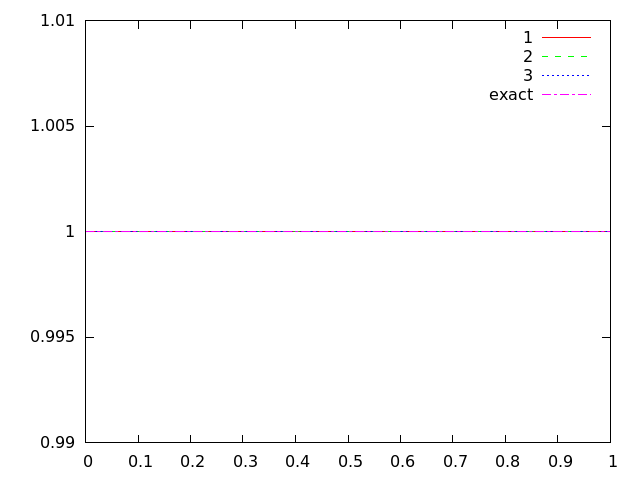
\includegraphics[width=.425\textwidth]{prs_T8.png} &
	  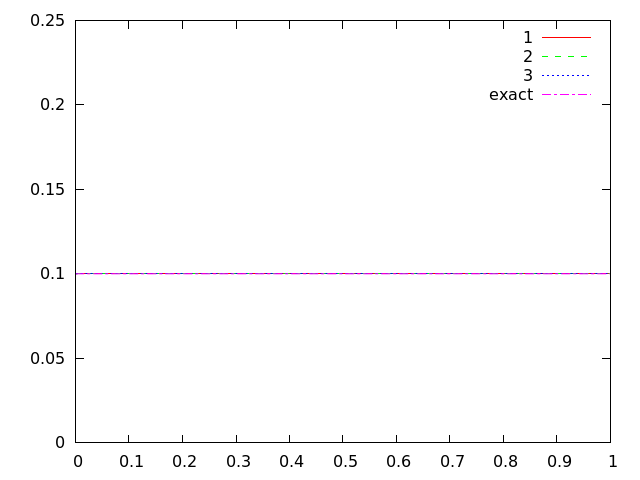
\includegraphics[width=.425\textwidth]{vel_T8.png}
	\end{tabular}
  \end{center}
  \caption{pressure and velocity}
\end{figure}

\clearpage

\subsection{Test 9}
When finding density, method 1 falls considerably short of the maximum. On the pressure graph, method 3 features both a jump above and a dip below the graph between positions 0.1 and 0.2. Velocity shows a similar (but considerably larger) dip, followed by jump, in the vertical section of the graph between 0.1 and 0.2. Method 1 also overestimates the maximum velocity and is above both exact and method 3 in the middle horizontal section. 

\begin{figure}[h]
  \begin{center}
	\begin{tabular}{cc}
      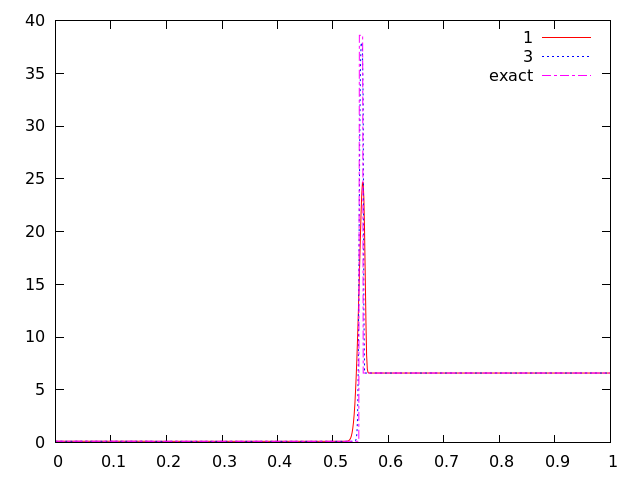
\includegraphics[width=.4\textwidth]{den_T9.png} &
	  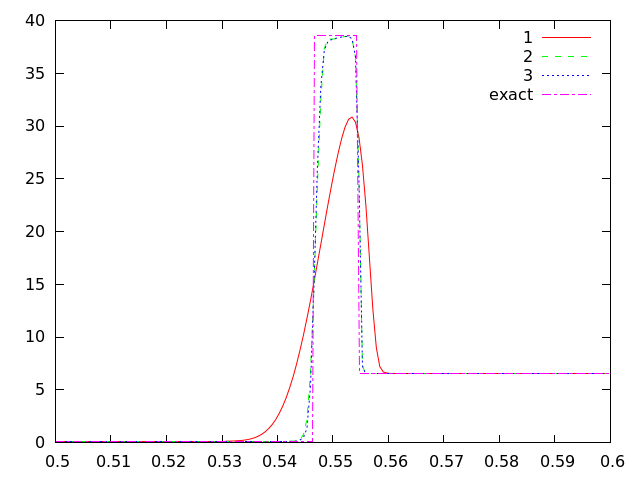
\includegraphics[width=.4\textwidth]{denT9zoom.png} \\
	  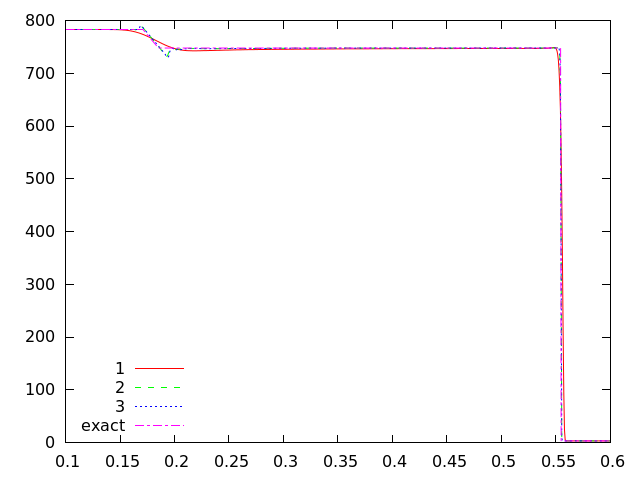
\includegraphics[width=.4\textwidth]{prs_T9.png} &	
      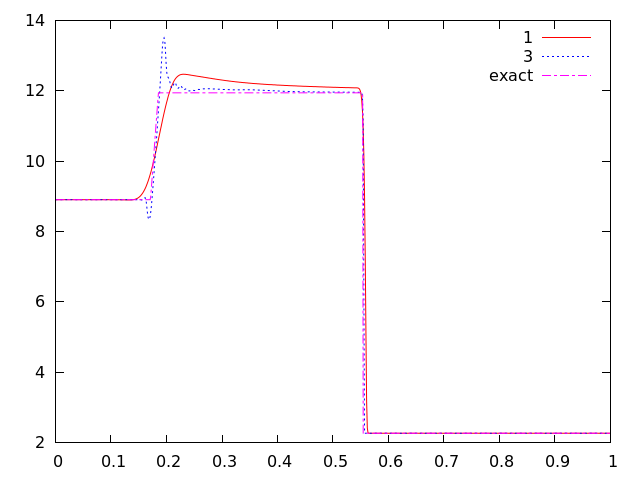
\includegraphics[width=.4\textwidth]{vel_T9.png}\\
	\end{tabular}	
  \end{center}
  \caption{}
\end{figure}

\begin{figure}[h]
  \begin{center}
     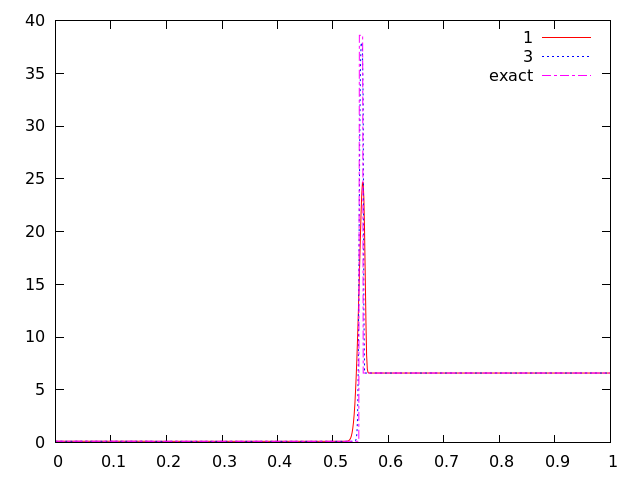
\includegraphics[width=.78\textwidth]{den_T9.png}	
  \end{center}
  \caption{density}
\end{figure}

\begin{figure}
  \begin{center}
     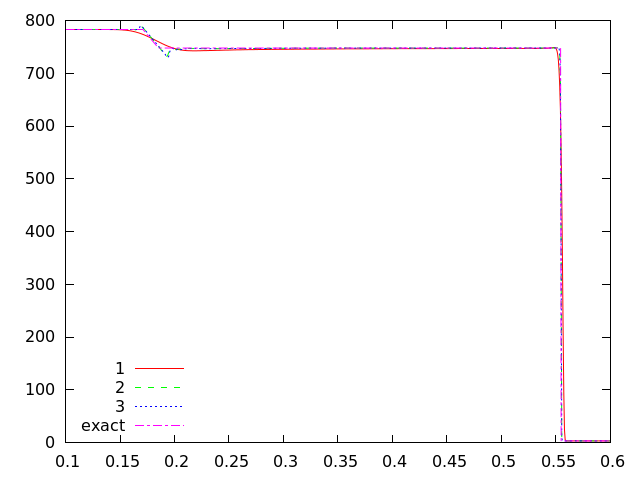
\includegraphics[width=.78\textwidth]{prs_T9.png}	
  \end{center}
  \caption{pressure}
\end{figure}

\begin{figure}
  \begin{center}
     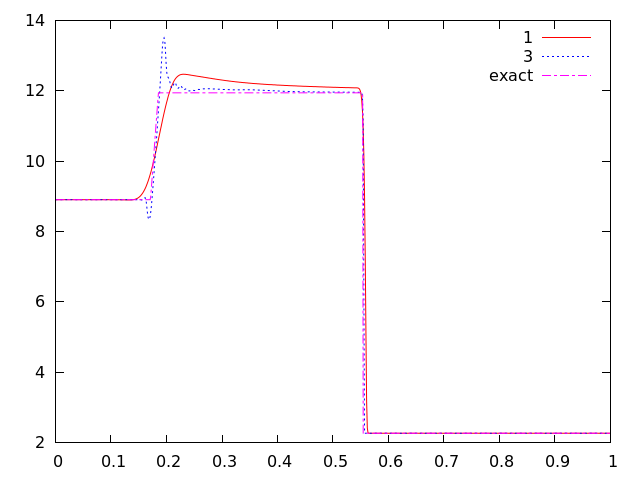
\includegraphics[width=.78\textwidth]{vel_T9.png}	
  \end{center}
  \caption{velocity}
\end{figure}
\clearpage

\subsection{Test 10}

\begin{figure}[h]
  \begin{center}
	\begin{tabular}{cc}
      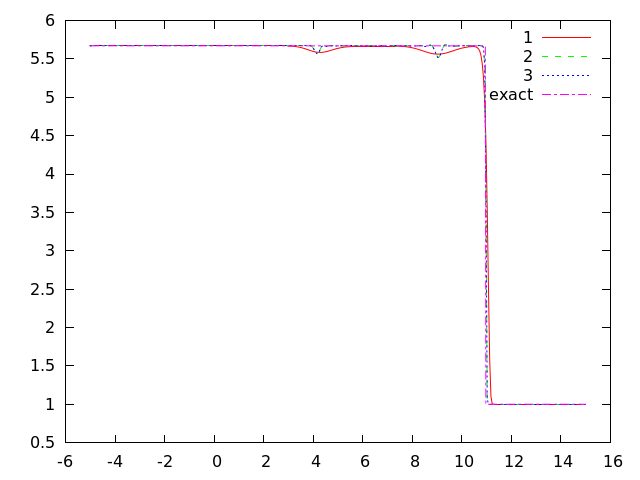
\includegraphics[width=.4\textwidth]{den_T10.png} &
	  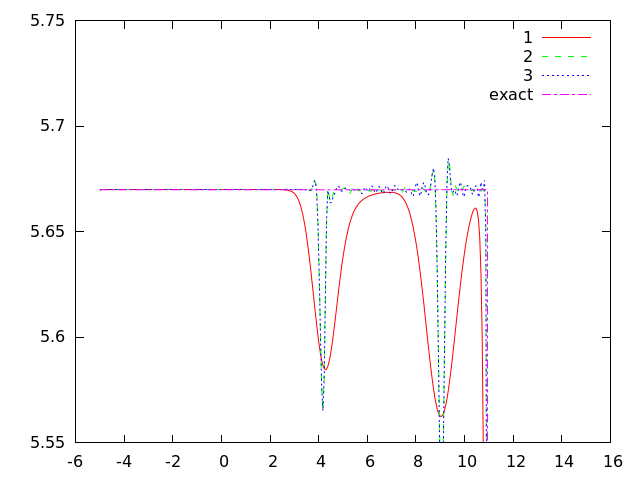
\includegraphics[width=.4\textwidth]{den10zoom.png} \\
	  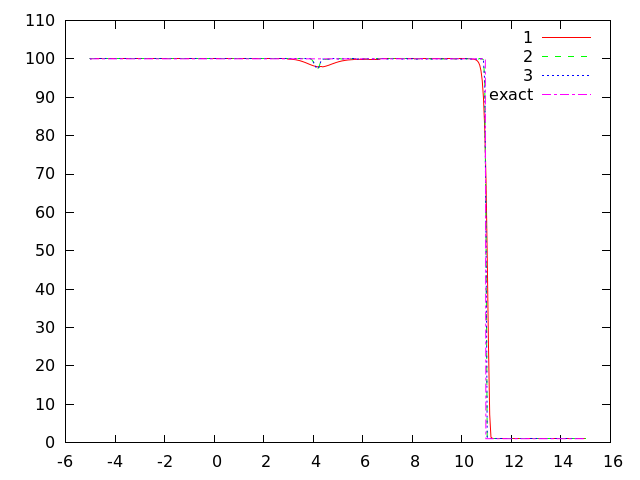
\includegraphics[width=.4\textwidth]{prs_T10.png} &	
	  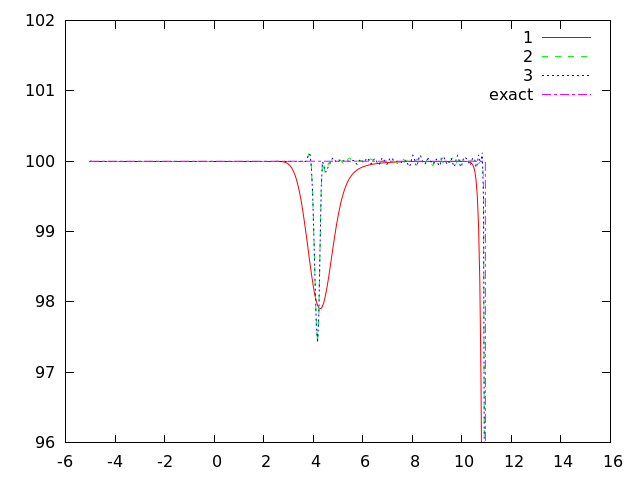
\includegraphics[width=.4\textwidth]{prs10zoom.png} \\
      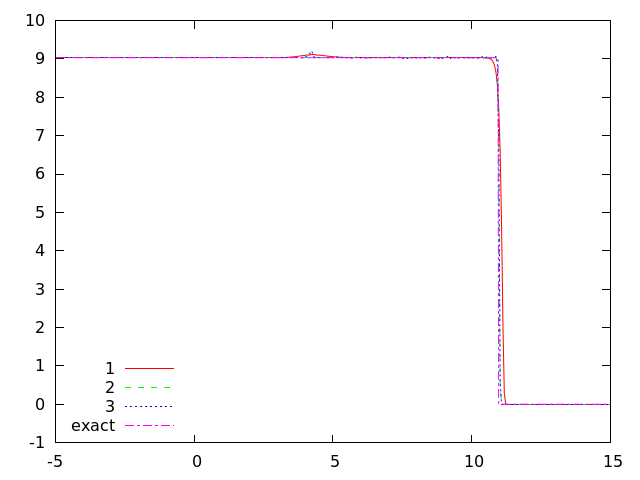
\includegraphics[width=.4\textwidth]{vel_T10.png} &	
      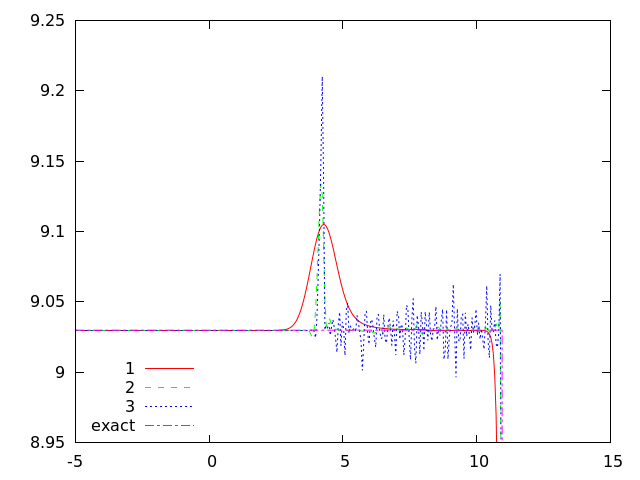
\includegraphics[width=.4\textwidth]{vel10zoom.png} \\
	\end{tabular}	
  \end{center}
  \caption{}
\end{figure}



\clearpage

\subsection{Test 11}

\begin{figure}[h]
  \begin{center}
	\begin{tabular}{cc}
      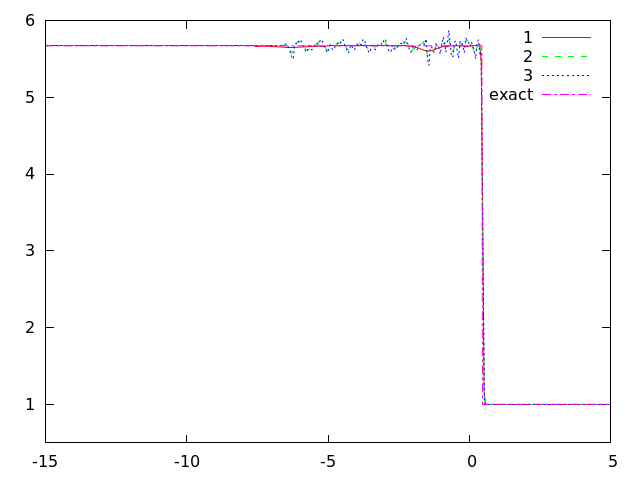
\includegraphics[width=.4\textwidth]{den_T11.png} &
	  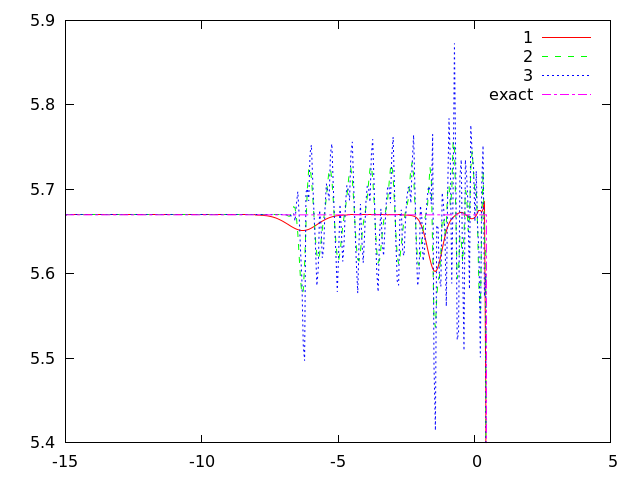
\includegraphics[width=.4\textwidth]{den11zoom.png} \\
	  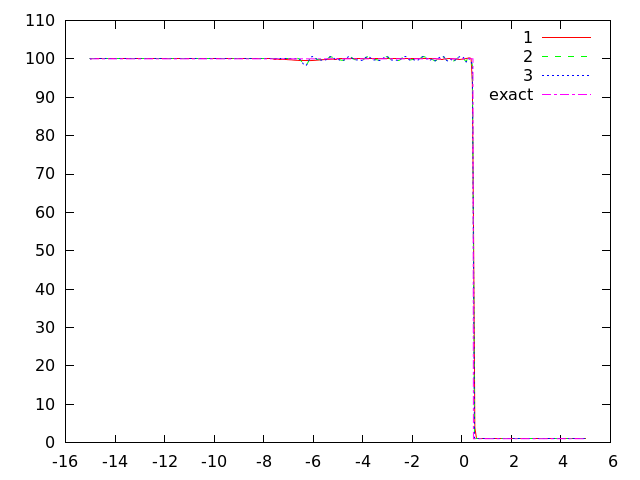
\includegraphics[width=.4\textwidth]{prs_T11.png} &	
	  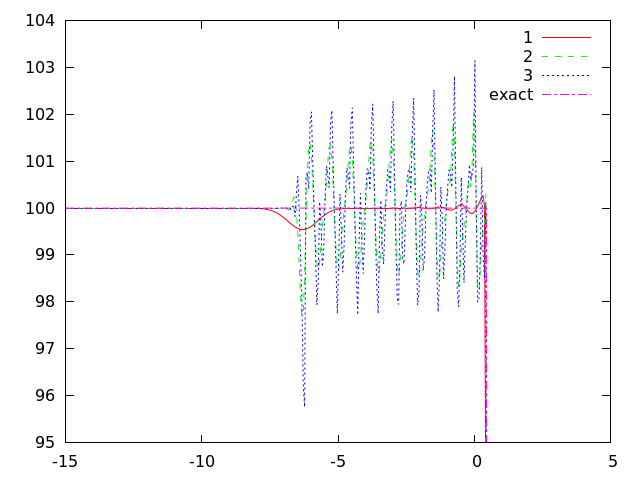
\includegraphics[width=.4\textwidth]{prs11zoom.png} \\
      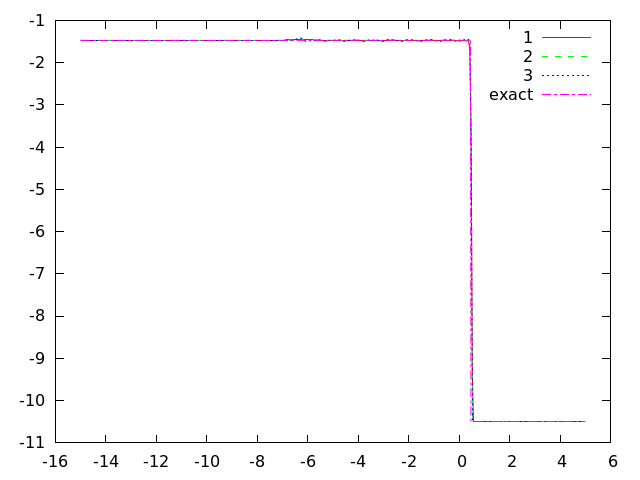
\includegraphics[width=.4\textwidth]{vel_T11.png} &	
      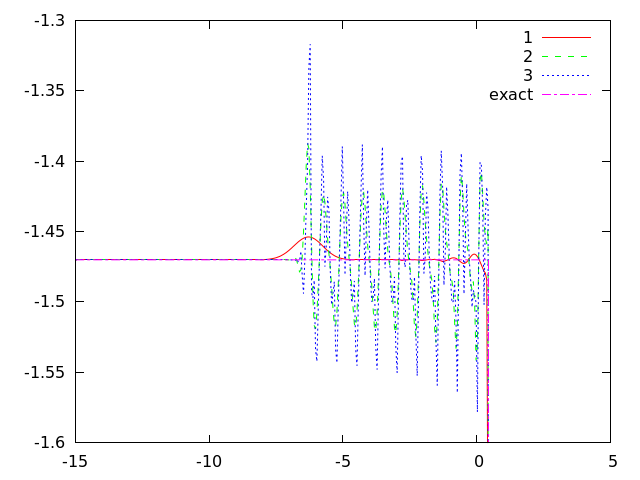
\includegraphics[width=.4\textwidth]{vel11zoom.png} \\
	\end{tabular}	
  \end{center}
  \caption{}
\end{figure}

\clearpage

\subsection{Test 12: Interacting Blast Waves}
This test was run for all three integration methods with both 400 cells and 2000 cells. Since it has no exact solution, the 2000 cell, third order test is compared to all three 400 cell tests and labeled as ``exact.''

\begin{figure}[h]
  \begin{center}
     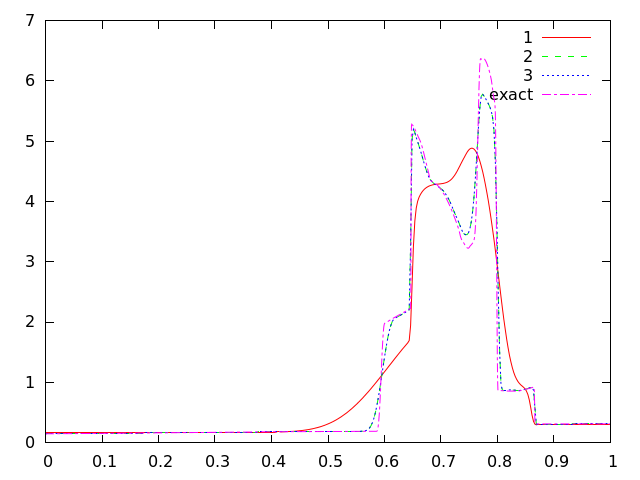
\includegraphics[width=.78\textwidth]{den_T12_400.png}	
  \end{center}
  \caption{density (400 cells)}
\end{figure}

\begin{figure}[h]
  \begin{center}
     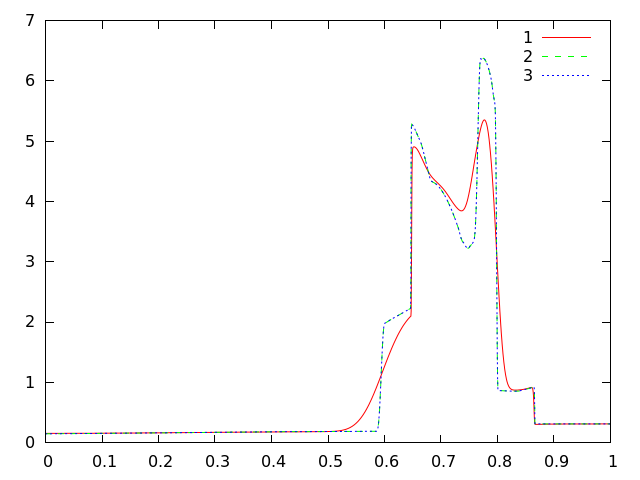
\includegraphics[width=.78\textwidth]{den_T12_2000.png}	
  \end{center}
  \caption{density (2000 cells)}
\end{figure}

\begin{figure}[h]
  \begin{center}
     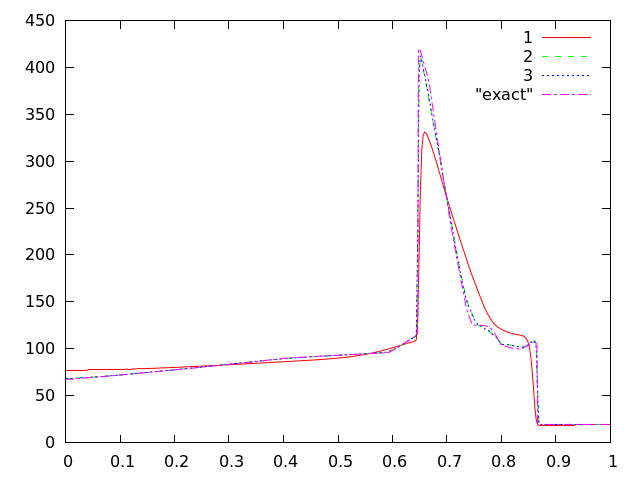
\includegraphics[width=.78\textwidth]{prs_T12_400.png}	
  \end{center}
  \caption{pressure (400 cells)}
\end{figure}

\begin{figure}[h]
  \begin{center}
     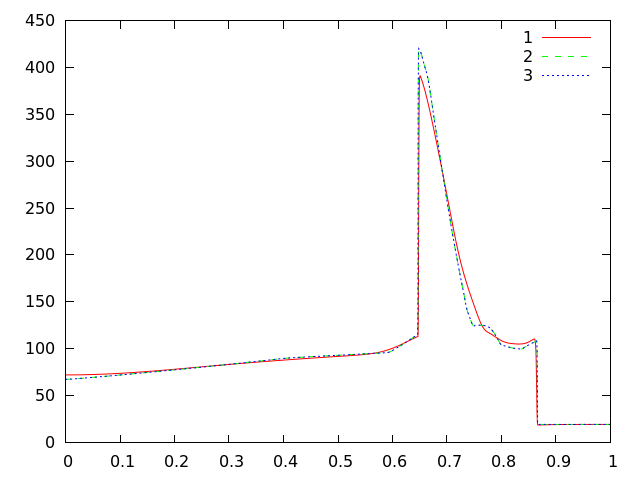
\includegraphics[width=.78\textwidth]{prs_T12_2000.png}	
  \end{center}
  \caption{pressure (2000 cells)}
\end{figure}

\begin{figure}[h]
  \begin{center}
     \includegraphics[width=.78\textwidth]{vel_T12_400.png}	
  \end{center}
  \caption{velocity (400 cells)}
\end{figure}

\begin{figure}[h]
  \begin{center}
     \includegraphics[width=.78\textwidth]{vel_T12_2000.png}	
  \end{center}
  \caption{velocity (2000 cells)}
\end{figure}

\bibliographystyle{siam}
\bibliography{references.bib}

\end{document}
